\section{Data, Monte Carlo, and HGam Pre-selection} \label{sec:DataMC}

\subsection{Data} \label{sec:Data}

In both Run-2 HGam analyses discussed in this dissertation, we use the full LHC Run-2 dataset, consisting of $139.0 \pm 2.4 fb^{-1}$ of proton-proton collisions with a center of mass energy $\sqrt{s} = 13 TeV$ recorded by the ATLAS detector between 2015 and 2018 \ref{ATLAS-CONF-2019-021}. Figure \ref{fig:datalumi} shows the instantaneous luminosity gathered by the detector as a function of time; figure \ref{fig:pileup} shows the number of pileup events per bunch-crossing as a function of time. 

\begin{figure}
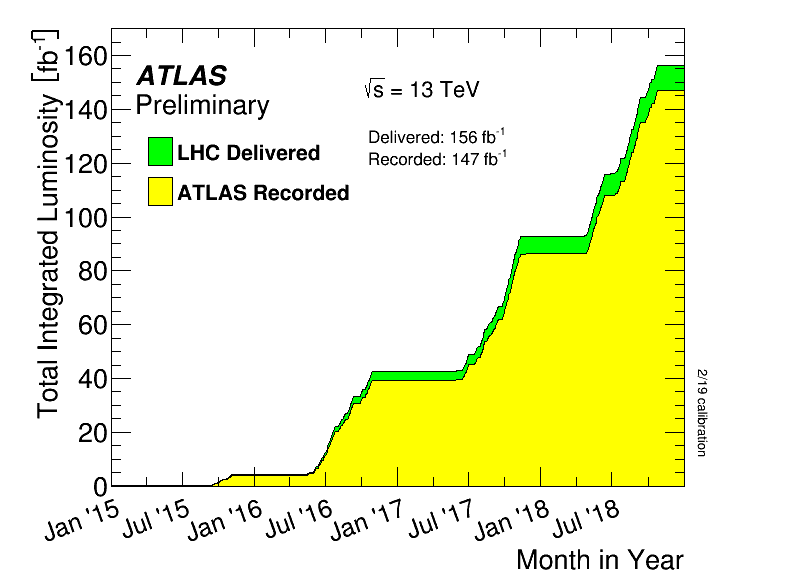
\includegraphics[width=0.5\linewidth]{figures/datamc_chapter/datalumi.png}
\caption{Integrated luminosity for the Run-2 ATLAS data-taking period.}
\end{figure}

\begin{figure}
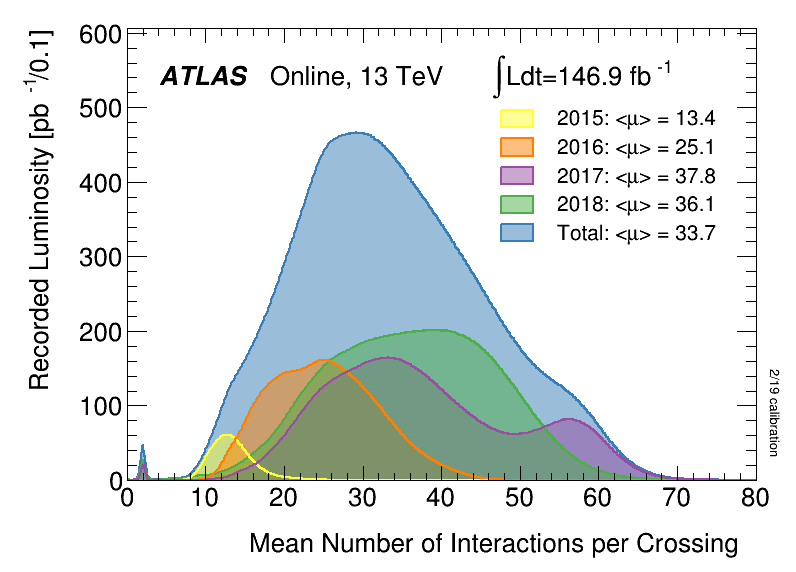
\includegraphics[width=0.5\linewidth]{figures/datamc_chapter/pileup.png}
\caption{Pileup for the Run-2 ATLAS data-taking period.}
\end{figure}

The trigger used to select events is the diphoton trigger HLT\_g35\_loose\_g25\_loose (for 2015-2016 data) and HLT\_g35\_medium\_g25\_medium (for 2017-2018 data). Both triggers require two photon candidates, one with a transverse energy $E_{T}$ of at least 35 GeV and the other with transverse energy of at least 25 GeV. The 2015-2016 trigger requires two photons that pass the "loose" ID requirement, while the 2017-2018 trigger requires two photons that pass the "medium" ID requirement (the cut was tightened due to increased luminosity and pileup). The trigger was calibrated using radiative Z decays, and is observed to be greater than 95\% efficient for each photon as long as it is 5 GeV above the trigger threshold \ref{cite:TriggerPerformance}.

\begin{figure}
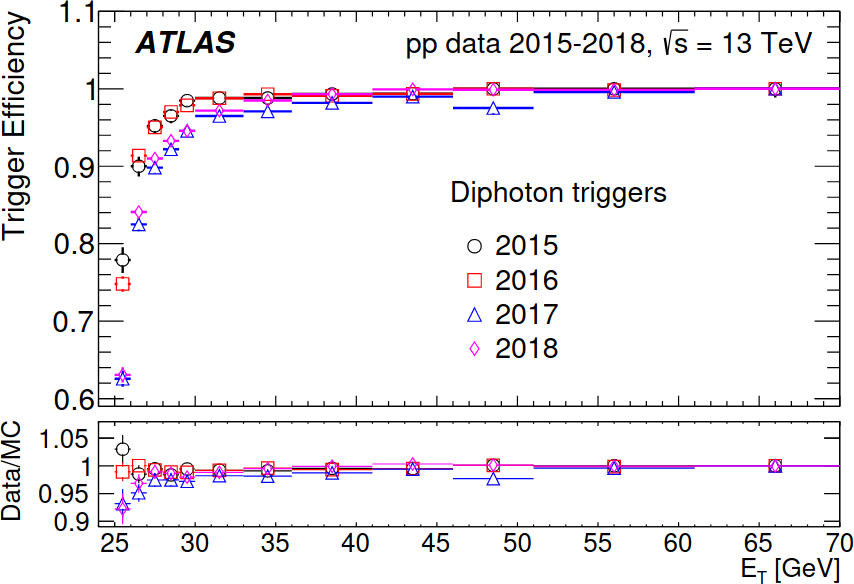
\includegraphics[width=0.5\linewidth]{figures/datamc_chapter/trigger.png}
\caption{Efficiency of the trigger for the different years of the run-2 data taking period as a function of subleading photon $E_{T}$.}
\end{figure}

\subsection{Higgs Preselection and Data CRs} \label{sec:Preselection} 

In both analyses discussed in this dissertation, we use the following preselection to define the $H \rightarrow \gamma \gamma$ signal region. These requirements are applied for both data and Monte Carlo simulation. 

\begin{itemize}
\item $\gamma\gamma Preselection$: The event is required to contain two photons passing the loose isolation and ID requirements.
\item $PV$: At least one primary vertex is required to be identified in the event.
\item $Trigger-Matching$: The leading two photons observed are required to match those identified by the trigger.
\item $Relative p_{T}$: The leading and subleading photons are required to have $p_{T}/m\gamma\gamma$ larger than 0.35 and 0.25, respectively.
\item $TI$: For events in the signal-region, we require both photons to pass the "Tight" Photon ID and Isolation requirements (for events in the 'NTI' data control region, this selection criterion is ignored). 
\item $Invariant Mass$: The invariant mass of the diphoton system must satisfy $105 GeV < m_{\gamma\gamma} < 160 GeV$
\end{itemize}

In order to accurately model the continuum diphoton background, it is often useful to invert the $TI$ requirement- that is, we construct a data sample consisting of those events passing all other preselections, but for which one or more photons does not pass either or both of the "tight" isolation and ID requirements. Data control samples in this not-tight-isolated "$NTI$" region allow us to model the kinematic properties of objects in the event other than the diphoton system, such as top quark jet variables, with some amount of accuracy.

Additionally, it is useful to consider the $TI$ or $NTI$ data sidebands- this consists of the set of events passing either $TI$ or $NTI$ selection in the region $105 GeV < m_{\gamma\gamma} < 160 GeV$ but outside the signal region ($123 GeV < m_{\gamma\gamma} < 127 GeV$ for the CP analysis, $120 GeV < m_{\gamma\gamma} < 130 GeV$ for the Couplings analysis). This allows us to model the shape of the background while safely away from the Higgs signal peak near 125 GeV. This is detailed further in the subsequent analysis-specific chapters.

\subsection{Nominal and Alternative Monte Carlo Samples} \label{sec:NominalMC} 

In order to generate Monte Carlo simulated events, several software programs must work in concert. In a real physics event, different proton constituents (usually gluons or quarks, often called "partons"), interact with one another in a process called a hard scatter to produce new particles. 

To simulate such a collision, the quantum field-theoretic "matrix element" that governs the dynamics of the hard-scatter process must be calculated, the momentum distributions of the individual partons must be modelled using Parton Distribution Functions (or PDFs), and the decay showers of any final-state hadrons produced in the event must be dynamically modelled. Additionally, the dynamics of proton constituents not contributing to the hard scatter, called the "underlying event", must also be simulated. Because showering and underlying event processes are difficult to accurately model, they are "tuned" on the data using a variety of particular parameter sets \ref{cite:tunes}. 

The Monte Carlo samples used in this dissertation are constructed using either the $MadGraph5\_aMC@NLO 8.2.12$ \ref{cite:MG5} \ref{cite:aMCNLO} or Powheg 7.03 \ref{cite:Powheg1} \ref{cite:Powheg2} \ref{cite:Powheg3} generators for matrix element calculation, Pythia8v2 \ref{cite:Pythia1} \ref{cite:Pythia2} or Herwig7v2.6.2 \ref{cite:Herwig1} \ref{cite:Herwig2} for showering, EvtGen 1.1 for hadronization of final-state jets \ref{cite:EvGen}, and Sherpa 1.2.0 \ref{cite:Sherpa1} \ref{cite:Sherpa2} \ref{cite:Sherpa3} \ref{cite:Sherpa4} for the matrix element calculation, showering, and hadronization of certain high-statistics samples.

After generation, Monte Carlo simulations are then passed through the Geant4 software package \ref{Geant4} to simulate the detector response. After this, the events are passed through the same object-reconstruction software used for data events \ref{cite:arXiv.1005.4568}. All Monte Carlo samples used in this dissertation are generated using the Geant4 full simulation, with the exception of the QCD continuum diphoton samples used for background modelling, which were treated using the GEANT4 fast simulation settings due to the number of events generated. For all MC samples, pile-up interactions were simulated by overlaying each Monte Carlo event with a different number of minimum-bias events simulated using Pythia 8.186 \ref{cite:Pythia} with the ATLAS "A3" tune \ref{cite:A3}.

In all Monte Carlo simulations, the Higgs mass was set to 125 GeV and the decay width was set to 4.07MeV \ref{cite:HiggsWidth}. All samples described include the small contribution from Dalitz decays (that is, decays in which one photon converts into two real final-state leptons), which is accounted for in the normalization of the samples. For all Monte Carlo samples generated using Madgraph5\_aMC@NLO, the renormalization ($\mu_{R}$) and factorization ($\mu_{F}$) scales are defined as the scalar sum of the transverse masses of all final-state particles divided by two (i.e. $H_{T}/2$), and the top and W boson decays are handled by MadSpin \ref{cite:MadSpin} in order to ensure the correct treatment of the spin correlations of the decay products.

For all simulated samples, several corrections are applied to ensure the simulated samples correspond to data, including a beam-spot width correction, photon shower-shape and calorimetric isolation corrections, energy scale and resolution corrections, photon identification and isolation corrections, jet selection efficiency corrections, and electron and muon identification, reconstruction and isolation corrections.

\begin{table}[h!]
  \centering
  \resizebox{\columnwidth}{!}{%
	\begin{tabular}{ |c|c|c|c| }
    	Prod. Mode   &      Generator       & PDF (Matrix Element) & PDF+Tune (Parton Shower)\\ 
		\hline
		    \ggF    &  \NNLOPS + \PYTHIA   & \PDFLHC  &  AZNLOCTEQ6   \\
			\VBF    &      \POWPYTHIA      & \PDFLHC  &  AZNLOCTEQ6   \\
  			$W^{+}H$  &      \POWPYTHIA      & \PDFLHC  &  AZNLOCTEQ6   \\
			$W^{-}H$  &      \POWPYTHIA      & \PDFLHC  &  AZNLOCTEQ6   \\
			$qq\to ZH$ &      \POWPYTHIA      & \PDFLHC  &  AZNLOCTEQ6   \\
			$gg\to ZH$ &      \POWPYTHIA      & \PDFLHC  &  AZNLOCTEQ6   \\
			\bbH    &      \POWPYTHIA      & \PDFLHC  &  A14NNPDF23   \\
			\ttH    &      \POWPYTHIA      & \PDFLHC  &  A14NNPDF23   \\
			\ttH    & \MGMCatNLO + \PYTHIA &  \NNPDF  &  A14NNPDF23   \\
			\tHbj   & \MGMCatNLO + \PYTHIA &  \NNPDF  &  A14NNPDF23   \\
			\tHW    & \MGMCatNLO + \PYTHIA &  \NNPDF  &  A14NNPDF23   \\
			
		\hline
	\end{tabular}
	}
  \caption{Summary of nominal signal samples}
  \label{tab:signal_samples_pyt}
\end{table}

Nominal gluon-gluon fusion events are simulated using the Powheg NNLOPS tool \ref{cite:NNLOPS} using the PDF4LHC15 PDF set \ref{cite:PDF4LHC}, while the nominal $VBF$, $WH$, $ZH$, and $ggZH$ are all generated using the Powheg generator with the PDF4LHC15 PDF set. Showering is performed with Pythia using the AZNLO tune \ref{cite:AZNLO} and the CTEQ6 PDF set \ref{cite:CTEQ6} for these samples. Nominal Standard-Model $ttH$ and $bbH$ samples are generated using the PowhegBOX tool \ref{cite:PowhegBox} using the PDF4LHC15 PDF set; for these samples, showering is performed with Pythia using the A14 tune \ref{cite:A14} and the NNPDF23 PDF set \ref{cite:NNPDF23}. Nominal $tWH$ and $tHjb$ samples are generated using the Madgraph5\_aMC@NLO generator with the NNPDF30 PDF Set \ref{cite:NNPDF30}, and are showered using Pythia with the A14 tune and the NNPDF23 PDF set. $tWH$ samples are generated using the five-flavor PDF scheme, while $tHjb$ samples are generated using the four-flavor PDF scheme. At first order, NLO corrections to the $tWH$ process contain final-state bottom quark jets that thus lead to interference with the more-common $ttH$ process \ref{cite:DemartintWH}; to resolve this, a diagram subtraction method is used \ref{cite:subtraction}.
Additionally, a $ttH$ sample is generated using the Madgraph5\_aMC@NLO generator with the NNPDF30 PDF Set \ref{cite:NNPDF30} for use with the dedicated $ttH CP$ samples, in order to confirm the validity of the effective field theory model used to generate them.

Alternative Standard-Model samples are developed using Herwig for showering rather than Pythia, in order to evaluate the parton-showering uncertainty. The matrix element generators and PDFs are all the same as for the nominal samples, with the exception of the VBF sample, for which generator weights were unable to be included using the Herwig showering tool (and thus the NNPDF30 PDF is quoted for both the generator and the showering tool). $ggF$, $VBF$, $VH$, $tWH$, $tHjb$ and the supplementary Madgraph5\_aMC@NLO $ttH$ sample are all showered using the H7P1 Tune \ref{cite:H7p1}, and the Powheg $ttH$ sample is showered using the \ref{cite:H7UE} tune.

Additionally, a supplementary $ggF$ sample is generated using Madgraph5\_aMC@NLO containing an additional two partons at the matrix element stage. To avoid double-counting events with additional final-state partons, the "FxFx" merging scheme is employed. This sample is showered with Pythia using the NNPDF30 PDF and the A14 tune.
 
\begin{table}[h!]
  \centering
  \resizebox{\columnwidth}{!}{%
    \begin{tabular}{ |c|c|c|c| }
    	Prod. Mode   &      Generator       & PDF (Matrix Element) & PDF+Tune (Parton Shower)\\ 
    	\hline
		\ggF    &  \NNLOPS + \HERWIG   & \PDFLHC  &  \NNPDF+H7p1  \\
		\VBF    &  \POWHEG + \HERWIG   &  \NNPDF  &  \NNPDF+H7p1  \\
		$W^{+}H$  &  \POWHEG + \HERWIG   & \PDFLHC  &  \NNPDF+H7p1  \\
		$W^{-}H$  &  \POWHEG + \HERWIG   & \PDFLHC  &  \NNPDF+H7p1  \\
		$qq\to ZH$ &  \POWHEG + \HERWIG   & \PDFLHC  &  \NNPDF+H7p1  \\
		$gg\to ZH$ &  \POWHEG + \HERWIG   & \PDFLHC  &  \NNPDF+H7p1  \\
		\ttH    &  \POWHEG + \HERWIG   & \PDFLHC  &  \NNPDF+H7UE  \\
		\ttH    & \MGMCatNLO + \HERWIG &  \NNPDF  &  \NNPDF+H7p1   \\
		\tHbj    & \MGMCatNLO + \HERWIG &  \NNPDF  &     \NNPDF+H7p1      \\
		\tHW    & \MGMCatNLO + \HERWIG &  \NNPDF  &     \NNPDF+H7p1      \\
		\ggF    & \MGMCatNLO + \PYTHIA & \NNPDF   &     \NNPDF+A14       \\
    	\hline
    \end{tabular}
  }
  \caption{Summary of alternative signal samples}
  \label{tab:signal_samples_herwig}
\end{table}  

The cross-sections for all Higgs processes are normalized to the state-of-the-art precision measurements discussed in \ref{cite:YellowReport4} using K-factor scaling factors. The accuracy of the cross-sections is N3LO QCD $+$ NLO Electroweak for $ggF$, NNLO $QCD$ $+$ NLO Electroweak for $VBF$ and $VH$, and NLO QCD $+$ NLO Electroweak for $ttH$, while $tHjb$ and $tWH$ are produced at NLO QCD with no electroweak correction. Additionally, samples are normalized to account for the $H \rightarrow \gamma \gamma$ branching ratio of $2.270 \times 10^{-3}$ calculated with HDECAY \ref{cite:HDecay} and PROPHECY4F \ref{cite:Prophecy}.

\begin{table}[h!]
  \centering
  \resizebox{0.25\columnwidth}{!}{%
    \begin{tabular}{ c|l }
      Prod. Mode & {XSxBR [pb]}   \\
      \hline
    	 \ggF       & 0.1101404   \\
    	 \VBF       & 0.00857833  \\
    	 $W^{+}H$   & 0.00190226  \\
    	 $W^{-}H$   & 0.00120605  \\
    	 $qq\to ZH$ & 0.001724519 \\
    	 $gg\to ZH$ & 0.000278529 \\
    	 \ttH       & 0.001149755 \\
    	 \tHbj      & 0.00016857  \\
    	 \tHW       & 3.44359e-05 \\
         \bbH       & 0.00110390  \\
    	\hline
    \end{tabular}
  }
  \caption{Cross sections times branching ratio values used to normalize each production mode. The values correspond to the state-of-the-art predictions and are taken from the CERN Yellow Report \ref{cite:YellowReport4}.}
  \label{tab:signal_samples_norm}
\end{table}  

The background for $H \rightarrow \gamma \gamma$ events is generally treated as a smoothly-falling, continuous distribution in diphoton mass $m_{\gamma \gamma}$. It is comprised of non-Higgs events containing real final-state or initial-state radiated photons, as well as hadronic jets that behave like photons. To model this, a functional-form based data-driven method is used; however, Monte Carlo templates are nonetheless used to facilitate and validate the background modelling.

Both QCD continuum $\gamma\gamma$ +jets production and the various $V\gamma\gamma \rightarrow ll\gamma\gamma$ samples are simulated at leading order in QCD using the Sherpa event generator with the CT10 PDF set \ref{cite:CT10}. Showering is performed using the default Sherpa showering tool. 

$t\bar{t}\gamma\gamma$, one of the leading backgrounds in top-enriched regions, is simulated using Madgraph5\_aMC@NLO with the NNPDF30 PDF set. It is showered using Pythia and tuned using the A14 tune.


\begin{table}[h!]
  \centering
  \resizebox{\columnwidth}{!}{%
  \begin{tabular}{|c|c|c|c|c|}
  	 Prod. Mode   &      Generator       & PDF (Matrix Element) & Showering Tool & PDF+Tune (Parton Shower)\\ 
  	\hline
  	$\gamma\gamma+$0,1(NLO),2,3(LO), \myy $\in$ 50-90 \GeV  & \SHERPA & CT10 & \SHERPA & CT10\\
 $\gamma\gamma+$0,1(NLO),2,3(LO), \myy $\in$ 90-175 \GeV & \SHERPA & CT10 & \SHERPA & CT10\\
         $ee\gamma\gamma$; $\myy>\SI{80}{\GeV}$          & \SHERPA & CT10 & \SHERPA & CT10\\
       $\mu\mu\gamma\gamma$; $\myy>\SI{80}{\GeV}$        & \SHERPA & CT10 & \SHERPA & CT10\\
      $\tau\tau\gamma\gamma$; $\myy>\SI{80}{\GeV}$       & \SHERPA & CT10 & \SHERPA & CT10\\
      $\nu\nu\gamma\gamma$; $\myy>\SI{80}{\GeV}$         & \SHERPA & CT10 & \SHERPA & CT10\\
        $e\nu\gamma\gamma$; $\myy>\SI{80}{\GeV}$         & \SHERPA & CT10 & \SHERPA & CT10\\
       $\mu\nu\gamma\gamma$; $\myy>\SI{80}{\GeV}$        & \SHERPA & CT10 & \SHERPA & CT10\\
       $\tau\nu\gamma\gamma$; $\myy>\SI{80}{\GeV}$       & \SHERPA & CT10 & \SHERPA & CT10\\
            $t\bar{t}\gamma\gamma$ (noallhad)            & \MGMCatNLO & \NNPDF & \PYTHIA & \NNPDF+A14       \\
             $t\bar{t}\gamma\gamma$ (allhad)             & \MGMCatNLO & \NNPDF & \PYTHIA & \NNPDF+A14       \\ 
  	\hline
  \end{tabular}
  }
\caption{Summary of nominal background samples}
\label{tab:bckg_samples}
\end{table}  

\subsection{ttHCP Monte Carlo Samples} \label{sec:ttHCPMC} 

In the $ttH CP$ analysis, an Effective Field Theory (EFT) setting a cutoff scale of 1 TeV, below which no new BSM particles coupling to the Higgs exist, is used to generate Monte Carlo samples. The EFT used is the Higgs Characterization (HC) model \ref{cite: HC}, implemented in the MadGraph5\_aMC@NLO generator with the NNPDF30 PDF set. In all BSM samples generated, we use Pythia for showering with the NNPDF23 PDF set and the A14 PDF set.

As previously mentioned, the top-Higgs interaction term of the Lagrangian in the presence of CP-violation can be parameterized as

\begin{equation}
\mathcal{L} = \kappa_{t} g_{t} \bar{t} (cos(\alpha)+ sin(\alpha) i \gamma^{5} )th
\end{equation}

where $g_{t} = \frac{-m_{t}}{v} = \frac{-173.26 GeV}{246 GeV} = -0.703$ , $\kappa_{t}$ is the dimensionless coupling-strength term ($\kappa_{t}= 1$ in the Standard Model), and $\alpha$ is an angle that parameterizes the CP-mixing strength ($\alpha = 0$ in the Standard Model, $\alpha = \frac{\pi}{2}$ in the fully CP-odd case). The interpretation of the $H \rightarrow \gamma \gamma$ and $ggF$ dependence on $\alpha$ is handled in several different ways, as discussed in \ref{sec:ttHCPresults}.

As in the nominal case, $t\bar{t}H$ and $tWH$ samples are generated using the five-flavor scheme, while the four-flavor scheme is used for the $tHjb$ process. The Standard Model cross-sections and branching ratios for all process are normalized to those given in the CERN Higgs Yellow Report 4 \ref{cite:yellowreport}, in which fixed scales and the five-flavor scheme are used. Those cross-sections are calculated at NLO QCD accuracy (without electroweak correction) for the $tHjb$ and $tWH$ processes, while $t\bar{t}H$ is calculated at both NLO QCD and NLO Electroweak accuracies. $ggF+ 2 jets$ samples are also generated using the MadGraph5\_aMC@NLO generator as the $ggF$ cross-section varies with $\alpha$ and $\kappa_{t}$. To ensure that the W-boson Higgs Coupling is kept constant, $tWH$ samples are generated by treating cos$\alpha \times \kappa_{SM}$=1.


K-factors are then computed to scale the Higgs Characterization Monte Carlo cross-sections to the Yellow Report cross-sections. The obtained K-factors are shown to be similar for different CP mixing angles; thus, the K-factors derived for the SM case can be safely used for the various samples with different $\alpha$ values. 

\begin{table}[h!]
\centering
\begin{tabular}{|c|c|||c|c|}
\hline
$\kappa_{t}$ & $\alpha$\ & cos$\alpha$ & $\kappa_{SM}$\\
\hline
1 & 0(SM, CP-even) & 1 & 1 \\
1 & 15 & 0.965926 & 1.035276 \\
1 & 30 & 0.866025 & 1.154701 \\
1 & 45 (CP max mixing) & 0.707107 & 1.414214 \\
1 & 60 & 0.5 & 2 \\
1 & 75 & 0.258819 & 3.863703 \\
1 & 90 (CP-odd)  & 0.000001 & 10$^{6}$ \\
  \hline \hline
 -1 & 0 & 1 & 1 \\
 0.5 & 0 & 1 & 1 \\
 2 & 0 & 1 & 1 \\
 2 & 45 & 0.707107 & 1.414214 \\
\hline
\end{tabular}
\caption{Parameters used in the HC model in order to allow for CP-couplings only in the top quark sector while fixing the HWW coupling to its SM value by imposing cos$\alpha~\kappa_{SM}$=1. In the first set of samples, $\kappa_{t}$ is fixed to 1 and $\alpha$ is varied. In the second set, $\kappa_{t}$ is set to values different from 1. For $\alpha=90$; due to numerical precision, $\cos\alpha$ strictly equal to 0 can't be generated and thus a value approaching it ($10^{-6}$) and a defined value for kSM ($10^{6}$) are used.}
\label{tab:MCsamples_Parameters}
\end{table}

\begin{table}[h!]
  \centering
  \begin{tabular}{|c|c||c|c|c|c|}
    \hline
    \multicolumn{6}{|c|}{Cross-section (pb)} \\
    \hline \hline
    $\kappa_t$ & $\alpha$ & ttH & tHjb & tWH & ggF\\
    \hline
    1 & 0(SM, CP-even) & 0.458 & 0.0606 & 0.0167 & 14.1\\
    1 & 15 & 0.443 & 0.0636 & 0.0184 & --\\
    1 & 30 & 0.396 & 0.0743 & 0.0231 & --\\
    1 & 45 (CP max mixing)& 0.329 & 0.0958 & 0.0308 & 24.0\\
    1 & 60 & 0.265 & 0.1374 & 0.0422 & --\\
    1 & 75 & 0.217 & 0.1970 & 0.0563 & --\\
    1 & 90 (CP-odd) & 0.199 & 0.2707 & 0.0726 & 32.4\\
    \hline \hline
    -1 & 0 & -- & 0.6971 & 0.1490 & -- \\
    0.5 & 0 & -- & 0.0939 & 0.0148 & -- \\
    2 & 0 & -- & 0.2406 & 0.0924 & -- \\
    2 & 45 & -- & 0.2055 & 0.1095 & -- \\
    \hline
  \end{tabular}
  \caption{NLO cross-sections for the $t\bar{t}H$, $tHjb$, $tWH$, and $ggF$ processes for different CP-scenarios (see parameters in Table~\ref{tab:MCsamples_Parameters}). The top part refers to MC samples in which the $\kappa_{t}$ value is fixed to 1 and $\alpha$ is varied, while the bottom part refers to samples with $\kappa_{t}$ different from 1.}
  \label{tab:MCsamples_XS}
\end{table}

\begin{table}
  \centering
  \begin{tabular}{|c|c||c|c|c|c|}
    \hline
    \multicolumn{6}{|c|}{Normalized Cross-section(fb)} \\
    \hline \hline
    $\kappa_t$ & $\alpha$ & ttH & tHjb & tWH & ggF\\
    \hline
    1 & 0(SM, CP-even)  & 1.150 & 0.169 & 0.034 & 33.1 \\
    1 & 15              & 1.113 & 0.177 & 0.038 & -- \\
    1 & 30              & 0.995 & 0.207 & 0.048 & -- \\
    1 & 45 (CP max mixing)      & 0.827 & 0.266 & 0.064 & 53.7 \\
    1 & 60              & 0.666 & 0.382 & 0.087 & -- \\
    1 & 75              & 0.545 & 0.548 & 0.116 & -- \\
    1 & 90 (CP-odd)     & 0.500 & 0.753 & 0.150 & 74.4 \\
    \hline \hline
    -1 & 0    & -- & 1.980 & 0.307 & -- \\
    0.5 & 0   & -- & 0.264 & 0.030 & -- \\
    2 & 0     & -- & 0.666 & 0.190 & -- \\
    2 & 45    & -- & 0.570 & 0.226 & -- \\
    \hline
  \end{tabular}
  \caption{NLO cross-sections for the $t\bar{t}H$, $tHjb$, $tWH$, and $ggF$ processes for different CP-scenarios normalized with the K-factor and BR$(H\rightarrow\gamma\gamma)$. The top part refers to MC samples in which the $\kappa_{t}$ value is fixed to 1 and $\alpha$ is varied, while the bottom part refers to samples with $\kappa_{t}$ different from 1.}
  \label{tab:MCsamples_XS_norm}
\end{table}
